\documentclass[a4paper,12pt]{article}

\usepackage[T1]{fontenc}
\usepackage[english]{babel}
\usepackage[utf8]{inputenc}
\usepackage{geometry}
\usepackage{booktabs}
\usepackage{graphicx}
\usepackage{amsmath}
\usepackage{hyperref}
\usepackage{float}
\usepackage{tabularx}

\geometry{left=2.5cm, right=2.5cm, top=2.5cm, bottom=2.5cm}

\title{\textbf{Technical Report: Internal Ballistics Simulation of Rocket Motors}}

\author{Paweł Mikołajewski\\Comparative Analysis of Propulsion Systems}

\date{\today}

\begin{document}

\maketitle
\newpage

\tableofcontents
\newpage

\section{Introduction}

The purpose of this study is a comparative analysis of the thrust profiles of four rocket motor types: two solid-propellant motors (KNSB and APCP) and two hybrid motors (N$_2$O/Paraffin and N$_2$O/HTPB). The analysis is based on mathematical models employing numerical solutions of internal ballistics equations.

The primary assumption of the study was to compare different propellant configurations while maintaining a similar total impulse level of approximately 3000 Ns. This approach enables evaluation of the influence of propellant type and propulsion architecture on thrust characteristics, burn duration, structural requirements, and rocket applications without the dominant effect of total system energy.

The presented results are intended for comparative purposes and provide an assessment of the behavior of individual propulsion systems under similar energetic requirements.

\section{Methodology and Modeling Assumptions}

A number of simplifying assumptions were adopted to model the physical phenomena while maintaining computational efficiency.

\subsection{Physical Analysis and Model Validation}

The mathematical model includes:

\begin{itemize}

    \item \textbf{Dynamic mass and energy balance:} A differential equation for chamber pressure ($P_c$) accounting for the coupling between gas generation and nozzle mass flow.

    \item \textbf{Ignition modeling:} An exponential function providing realistic pressure rise during motor startup.

    \item \textbf{Hybrid motor coupling:} Dynamic variation of the O/F ratio and its influence on characteristic velocity ($C^*$).

    \item \textbf{Geometry evolution:} Continuous update of burning surface area and chamber volume during operation.

\end{itemize}

\subsection{Model Simplifications}

\begin{itemize}

    \item Constant $C^*$ for each propellant.
    \item Simplified grain geometry.
    \item Marxman regression law for hybrid fuel regression.
    \item Constant atmospheric pressure.
    \item Constant specific heat ratio $\gamma$.

\end{itemize}

\section{Simulation Results}

\begin{figure}[H]
    \centering
    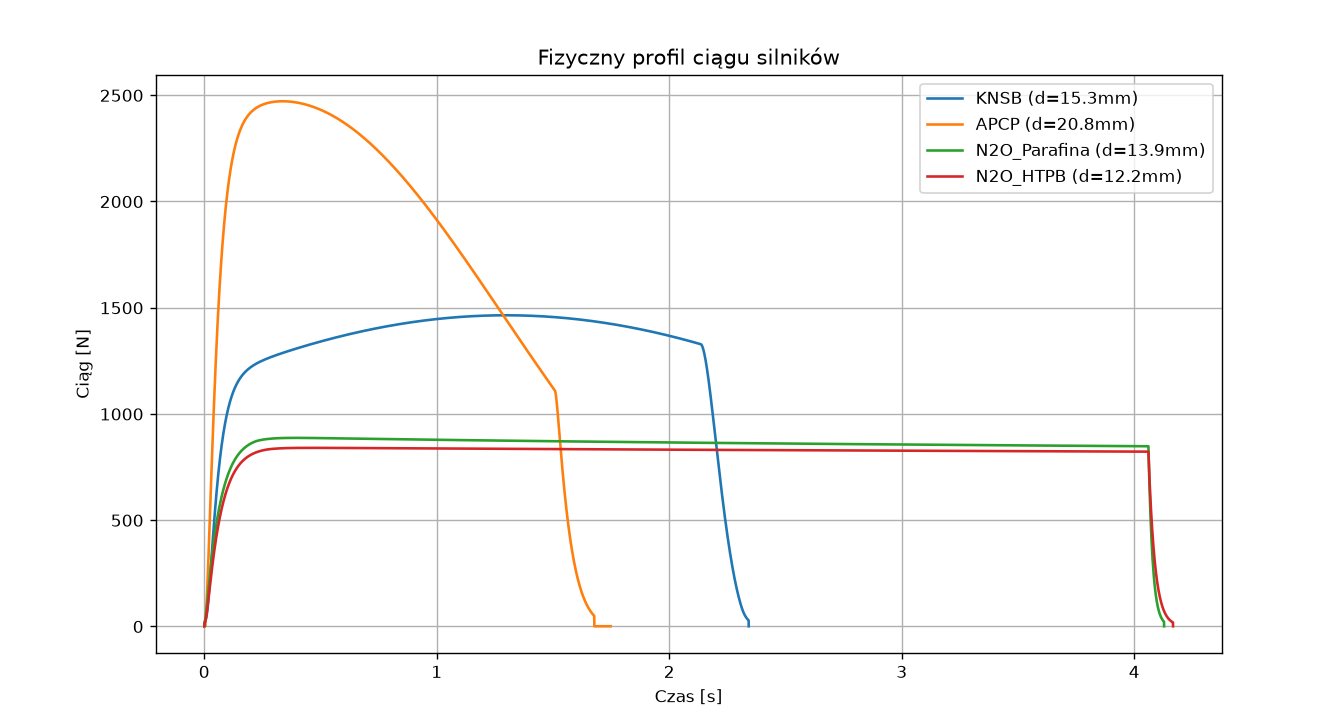
\includegraphics[width=0.9\textwidth]{comparison.png}
    \caption{Comparison of thrust profiles for the analyzed rocket motors}
    \label{fig:thrust_comparison}
\end{figure}

\begin{table}[H]
\centering
\caption{Summary of Design Parameters and Performance}

\begin{tabularx}{\textwidth}{lXXXX}
\toprule
\textbf{Motor} &
\textbf{Propellant Mass [kg]} &
\textbf{Total Impulse [Ns]} &
\textbf{Nozzle Diameter [mm]} &
\textbf{Burn Time [s]} \\
\midrule
KNSB & 2.44 & 2999 & 15.29 & approx. 2.2 \\
APCP & 1.45 & 3023 & 20.81 & approx. 1.6 \\
N$_2$O/Paraffin & 1.69 & 3476 & 13.87 & approx. 4.0 \\
N$_2$O/HTPB & 1.52 & 3339 & 12.20 & approx. 4.1 \\
\bottomrule
\end{tabularx}

\end{table}

\section{Results Analysis}

\subsection{Solid Propellant Characteristics}

APCP exhibits a very high and short-duration thrust pulse, whereas KNSB provides a more moderate and smoother combustion profile.

\subsection{Hybrid Motor Characteristics}

Hybrid motors offer longer burn durations and more stable thrust profiles.

\section{Conclusions}

The conducted analysis enabled a comparison of four propulsion configurations under the assumption of approximately 3000 Ns total impulse.

\begin{enumerate}

\item \textbf{Energy Efficiency}

Hybrid motors achieve higher utilization efficiency of propellant materials and longer burn durations at comparable total impulse levels.

\item \textbf{Thrust Profile}

APCP generates high initial thrust, KNSB provides a smoother profile, while hybrid motors exhibit the most stable thrust characteristics.

\item \textbf{Combustion Geometry}

Changes in burning surface area and O/F ratio significantly affect motor performance characteristics.

\item \textbf{Structural Requirements}

APCP requires the largest nozzle diameters and the highest thermal resistance of structural components.

\item \textbf{Safety}

Hybrid motors are inherently safer due to the physical separation of fuel and oxidizer.

\item \textbf{3000 Ns Design Assumption}

The comparison was performed at a similar total impulse level of approximately 3000 Ns, allowing assessment of the actual influence of propellant type on motor performance independently of the total system energy.

\end{enumerate}

\section{Future Work}

Further development of the model includes:

\begin{itemize}

\item variable $C^*$ model dependent on chamber pressure and gas composition,
\item integration with NASA CEA,
\item advanced grain geometry modeling,
\item erosive burning model,
\item N$_2$O tank dynamics model,
\item thermal losses and heat transfer modeling,
\item parameter sensitivity analysis,
\item experimental validation,
\item integration with a 6-DOF flight simulator.

\end{itemize}

The ultimate goal is to enable optimization of propellants for rocket motors with total impulse around 3000 Ns and the creation of a propulsion configuration database.

% --- REFERENCES ---
\begin{thebibliography}{9}

\bibitem{Sutton}
Sutton, G. P., Biblarz, O. (2016).
\textit{Rocket Propulsion Elements}.
Wiley.

\bibitem{Marxman}
Marxman, G. A., Woolridge, C. E., Muzzy, R. J. (1964).
\textit{Fundamentals of Hybrid Rocket Combustion}.

\bibitem{Huzel}
Huzel, D. K., Huang, D. H. (1992).
\textit{Modern Engineering for Design of Liquid-Propellant Rocket Engines}.

\end{thebibliography}

\end{document}